\begin{figure*}[!t]
  \center
  \def\layersep{2cm}
  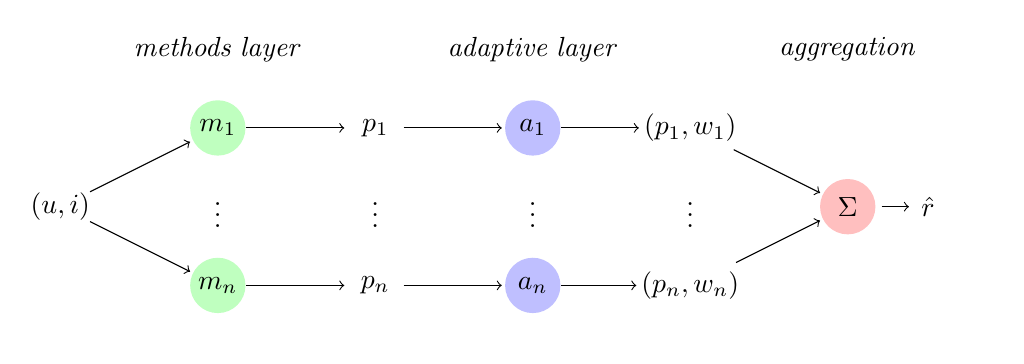
\begin{tikzpicture}[shorten >=1pt,->,draw=black, node distance=\layersep]

    \tikzstyle{every pin edge}=[<-,shorten <=2pt]
    \tikzstyle{node}=[circle,fill=black!25,minimum size=20pt,inner sep=0pt]
    \tikzstyle{input node}=[node, fill=green!25];
    \tikzstyle{output node}=[node, fill=red!25];
    \tikzstyle{hidden node}=[node, fill=blue!25];
    \tikzstyle{annot} = [text width=10em, text centered]
    \tikzstyle{txt}=[node,fill=white];
    
    \node[txt] (UI) at (0,-2) {$(u,i)$};  

    \node[input node] (I-1) at (\layersep,-1) {$m_1$};
    \node[txt]        (I-D) at (\layersep,-2) {$\vdots$};
    \node[input node] (I-N) at (\layersep,-3) {$m_n$};
    
    \node[txt] (P-1) at (\layersep*2, -1) {$p_1$};
    \node[txt] (P-D) at (\layersep*2, -2) {$\vdots$};
    \node[txt] (P-N) at (\layersep*2, -3) {$p_n$};

    \node[hidden node] (H-1) at (\layersep*3, -1) {$a_1$};    
    \node[txt]         (H-D) at (\layersep*3, -2) {$\vdots$};    
    \node[hidden node] (H-N) at (\layersep*3, -3) {$a_n$};    

    \node[txt] (R-1) at (\layersep*4, -1) {$(p_1,w_1)$};
    \node[txt] (R-D) at (\layersep*4, -2) {$\vdots$};
    \node[txt] (R-N) at (\layersep*4, -3) {$(p_n,w_n)$};
    
    % hidden helper node
    \node[txt] (HH)  at (\layersep*5,-1) {};

    % Draw the output layer node
    \node[output node,pin={[pin edge={->}]right:$\hat{r}$}] at (\layersep*5,-2) (O) {$\Sigma$};
    
    \path (UI) edge (I-1);
    \path (UI) edge (I-N);

    \path (I-1) edge (P-1);
    \path (I-N) edge (P-N);

    \path (P-1) edge (H-1);
    \path (P-N) edge (H-N);

    \path (H-1) edge (R-1);
    \path (H-N) edge (R-N);

    \path (R-1) edge (O);
    \path (R-N) edge (O);

    % Annotate the layers
    \node[annot,above of=I-1, node distance=1cm] {\emph{methods layer}};
    \node[annot,above of=H-1, node distance=1cm] {\emph{adaptive layer}};
    \node[annot,above of=HH,  node distance=1cm] {\emph{aggregation}};
  \end{tikzpicture}

  \vspace{1em}
  \caption[The Layers of Recommenders]{
    Layers of recommenders:
    The method layer consists of ordinary modeling methods,
    each predicting the rating between a user and an item.
    This produces a set of predicted ratings ($p$).
    The adaptive layer estimates how well each modeling method
    will perform for the current user and item,
    and weighs the predictions accordingly.
    This produces a set of predictions and weights [$(p,w)$].
    The aggregation weighs the predictions into a final score $\hat{r}$.  
  }
  \label{fig:adaptiveusermodeling}
\end{figure*}
